\documentclass[10pt, a4paper]{article}
\usepackage[utf8]{inputenc}

% Format
\setlength{\parindent}{0.5in}
\usepackage{layout}

% Font
\usepackage{MinionPro}
\input glyphtounicode
\pdfgentounicode=1
\usepackage{microtype}
\usepackage[super]{nth}

% Links
\usepackage[colorlinks=true, linkcolor=black, urlcolor=black, citecolor=black]{hyperref} 

% Language
\usepackage[british]{babel}

% References
\usepackage[bibnewpage, unnumberedbib]{apacite}

% Figures
\usepackage{graphicx}
\usepackage[small, labelfont=it, labelsep=period]{caption}

% Tables
\usepackage{booktabs}
\usepackage{ltablex}

% Frontmatter
\title{Protocol:\\\textit{Meta-analysis of the\\`ironic' effects of intergroup contact}}
\date{March 22, 2019}

\begin{document}
\maketitle

\begin{abstract}
\noindent This is the preregistered protocol for our meta-analysis of the relationship between intergroup contact and support for social change among members of disadvantaged groups. This protocol follows the PRISMA-P guidelines \cite{moher_prismap_2015, shamseer_prismap_2015} for preparing a systematic review protocol.
\end{abstract}

\section{Introduction}

\subsection{Rationale}
\label{sec:rationale}

In this meta-analysis, we are considering more than a decade of empirical research \cite{dixon_intergroup_2007} on the potential `ironic' \cite{saguy_irony_2009}, `sedative' \cite{cakal_investigation_2011}, or `demobilising' \cite{dovidio_reducing_2017} effects of intergroup contact. 

Prior research  mostly studied intergroup contact as a means to reduce prejudice and social conflict (for a meta-analysis, see \citeNP{pettigrew_meta_2006}). Most research on intergroup contact had studied members of advantaged or `majority' groups (for a meta-analysis, see \citeNP{tropp_meta_2005}). Reducing prejudice among advantaged-group members had been advocated as a way to reduce discrimination and to foster positive social change. Following initial theorising by \citeA{wright_strategic_2001}, \citeA{dixon_beyond_2005}, and \citeA{reicher_rethinking_2007}, researchers begun studying whether, in historically unequal societies, intergroup contact could instead \emph{hinder} social change by reducing support for social change among members of disadvantaged or `minority' groups. Since \citeauthor{dixon_intergroup_2007}'s \citeyear{dixon_intergroup_2007} first empirical test of this hypothesis, a growing number of studies have examined the relationships between intergroup contact and social change among disadvantaged-group members.

To date, this literature has been the subject of narrative reviews \cite<for example,>{mckeown_contact_2017}, but not of a systematic review or quantitative synthesis. Filling this gap, this protocol outlines a systematic review and meta-analysis of the so-called `ironic' effects of intergroup contact. This endeavour allows us to quantify the strength of the relevant relationships and to identify potential shortcomings of the available evidence.

\subsection{Objectives}
\label{sec:objectives}

In this meta-analysis, we examine the relevant literature to answer the following research questions:

\begin{enumerate}
\item [Q0] \emph{Does intergroup contact help or hinder social change?} For this review, we define social change as a reduction in social inequality that improves the situation of disadvantaged groups in a society. Though this question motivates our review, the meta-analysis will not conclusively answer whether, on balance, intergroup contact helps or hinders social change. By answering Q1--Q3, however, our review will test the most prominent hypotheses explaining how intergroup contact \emph{could} hinder social change.
\item [Q1] \emph{Does contact with advantaged-group members reduce collective action among dis\-ad\-vant\-aged-group members?} Our review uses \citeauthor{wright_collective_2010}'s \citeyear{wright_collective_2010} definition of collective action as any action taken to improve the ingroup's position in society. As such, collective action (by disadvantaged-group members) challenges the status quo and, if successful, improves the situation of the disadvantaged ingroup. To the extent that it prevents collective action, intergroup contact hinders social change.
\item [Q2] \emph{Does contact with advantaged-group members reduce dis\-ad\-vant\-aged-group members' support for policies that would benefit their ingroup?} Redistributive policies (for example, affirmative action) and similar initiatives can be important means to reduce social inequality. Members of disadvantaged groups, who stand to benefit from their implementation, are important advocates for these policies. To the extent that it reduces support for such policies, intergroup contact hinders social change.
\item [Q3] \emph{Does contact with advantaged-group members reduce perceptions of injustice among disadvantaged-group members?} Some researchers \cite<e.g.,>{saguy_irony_2009} suggest that intergroup contact could lull dis\-ad\-vant\-aged-group members into a false sense of equality. Being aware of the injustice faced by the ingroup, however, is an important prerequisite to instigating social change \cite{zomeren_toward_2008}. In addition, accurately perceiving the social reality is likely important to coping in a society marked by inequality. To the extent that it reduces perceptions of injustice, intergroup contact hinders social change.
\end{enumerate}

\noindent For Q1--Q3, we explore the following questions:

\begin{enumerate}
\item [QA]	\emph{What is the direction of the relationship between intergroup contact and the outcome variable?}
\item [QB]	\emph{How strong is the relationship between intergroup contact and the outcome variable?}
\item [QC]	\emph{How much does the relationship vary across study designs, measures, and settings?}
\end{enumerate}

\noindent Beyond the meta-analysis, we use the information collected on each study to review the quality of the available evidence and to identify gaps and limitations in the literature. Below, we describe the methods used to find, describe, and synthesise relevant studies.

\section{Methods}

\subsection{Eligibility criteria}
\label{sec:eligibility-criteria}

In this meta-analysis, we are considering studies that \textit{i.} included \textbf{participants} of a relatively disadvantaged group, see \emph{Types of participants}, that \textit{ii.} manipulated or measured \textbf{intergroup contact} with a relatively advantaged group, see \emph{Types of predictor variables}, and that \textit{iii.} measured \textbf{one or more} of: \textbf{collective action} (intentions), \textbf{support for policies} that benefit or harm the participants' ingroup, and/or perceptions or expectations of \textbf{injustice}, see \emph{Types of outcome variables}. Below, we discuss these criteria in detail.

\subsubsection{Types of studies}
We include quantitative studies of all designs, as long as they fulfil the criteria laid out above. We consider study design features as possible moderators of study effect size.

\subsubsection{Types of participants}
We include samples of participants whose ingroup is disadvantaged (in terms of status, power, and/or resources) relative to the outgroup they have (or report to have) contact with.

\subsubsection{Types of predictor variables}
\label{sec:predictor-variables}

We include studies if they measure or manipulate the quantity of, quality of, and opportunity for contact with members of outgroups that are relatively advantaged (in terms of status, power, and/or resources) compared to the participants' ingroup (see \emph{Types of participants}). We consider both positive and negative contact, where both are measured. We consider opportunity for contact, as it is a potential precursor to face-to-face contact, but not imagined or indirect contact.

\subsubsection{Types of outcome variables}
\label{sec:outcome-variables}

We include studies that measure \textbf{at least one} of the following outcome variables:

\begin{description}
\item[Collection action.] We consider measures of observed, reported, or intended engagement in any action aimed at improving the position of the participants' ingroup in society, including participating in protests, signing petitions, and other forms of violent or non-violent collective action. 
\item[Policy support.] We consider studies that measure support for policies and initiatives designed to improve the position the participants' ingroup in society.
\item[Perceived injustice.] We consider studies that measure perceptions that one is discriminated against because of one's group membership, that one's group faces discrimination in society, that one's group is relatively deprived compared to other groups, or that the deprivation and/or discrimination faced by one's group is unjust/illegitimate. We also consider expectations of fair treatment as the reverse of perceived injustice. We include studies that measure \textit{personal} and/or \textit{group} discrimination or a mixture of both.
\end{description}

\subsubsection{Other criteria}

We do not use any other criteria for eligibility for the meta-analysis.

\subsection{Information sources}
\label{sec:information-sources}

To find relevant studies, we retrieve records from electronic databases, including \emph{Scopus}, an abstract and citation database of peer-reviewed literature, the \emph{Scopus} secondary documents database\footnote{``A secondary document is a document that has been extracted from a Scopus document reference list but is not available directly in the Scopus database since it is not indexed by Scopus.''}, and \emph{PsycINFO}, an abstract database of psychological literature. We also search the \emph{ProQuest Dissertations and Theses} database for relevant grey literature. To find unpublished studies, we have sent a call for unpublished research to the mailing lists of the \emph{European Association of Social Psychology} and the \emph{Society for Personality and Social Psychology} (June/July, 2017). We send another call for unpublished research closer to publication in which we also include the mailing lists of the \emph{International Society of Political Psychology}, the \emph{Society for the Psychological Study of Social Issues}, and the \emph{Society of Australasian Social Psychologists}. To achieve more complete coverage, we retrieve records that cite, or are cited by, the included studies. We also identify experts in the field and send a list of included studies to them, asking for any studies we have missed. We consider all relevant studies published before \textbf{April 1, 2019}, as well as all unpublished studies. We update our database searches \textbf{every four months} until we submit our manuscript for publication.

\subsection{Search strategy}
\label{sec:search-strategy}

We developed a search strategy for locating studies that include the relevant predictor and outcome measures. We search titles, abstract, and keywords for relevant terms in four electronic databases. We search for relevant records in the \emph{Scopus} database using the following search terms:
\small
\begin{enumerate}
\item TITLE-ABS-KEY(*group AND (contact OR friendship) AND (``collective action'' OR protest OR ``collective behavio*r'' OR ``political behavio*r'' OR ``social change'' OR ``social justice''))
\item TITLE-ABS-KEY(*group AND (contact OR friendship) AND (policy OR policies OR ``affirmative action'' OR (politi* W/15 attitude*) OR (politi* W/15 preferenc*)) AND (redistribut* OR reparati* OR inequalit* OR equalit* OR injustice* OR justice* OR disadvantage* OR advantage* OR minorit* OR majorit*))
\item TITLE-ABS-KEY((contact OR friendship) AND (``perceived discrimination'' OR ``perceived *advantage'' OR ``relative deprivation'' OR ``group discrimination'' OR ``personal discrimination'' OR ``group deprivation'' OR ``perception* of discrimination'' OR ``perception* of group discrimination'' OR ``perception* of personal discrimination'' OR ``rac* discrimination''))
\end{enumerate}
\normalsize
We use the same terms to retrieve relevant records from the \emph{Scopus} secondary documents database. We retrieve relevant records from \emph{PsycINFO} using similar search terms:
\small
\begin{enumerate}
\item (``*group'' AND (contact OR friendship) AND (``collective action'' OR protest OR ``collective behavio*r'' OR ``political behavio*r'' OR ``social change'' OR ``social justice'')).ti,ab,id.
\item (``*group'' AND (contact OR friendship) AND (policy OR policies OR ``affirmative action'' OR (politi* AND attitude*) OR (politi* AND preferenc*)) AND (redistribut* OR reparati* OR inequalit* OR equalit* OR injustice* OR justice* OR disadvantage* OR advantage* OR minorit* OR majorit*)).ti,ab,id.
\item ((contact OR friendship) AND (``perceived discrimination'' OR ``perceived *advantage'' OR ``relative deprivation'' OR ``group discrimination'' OR ``personal discrimination'' OR ``group deprivation'' OR ``perception* of discrimination'' OR ``perception* of group discrimination'' OR ``perception* of personal discrimination'' OR ``rac* discrimination'')).ti,ab,id.
\end{enumerate}
\normalsize
We search for grey literature in the \emph{ProQuest Dissertations and Theses} database using the following search terms:
\small
\begin{enumerate}
\item NOFT(group AND (contact OR friendship) AND (``collective action'' OR protest OR ``collective behavio*r'' OR ``political behavio*r'' OR ``social change'' OR ``social justice''))
\item NOFT(group AND (contact OR friendship) AND (policy OR policies OR ``affirmative action'' OR (politi* N/15 attitude*) OR (politi* N/15 preferenc*)) AND (redistribut* OR reparati* OR inequalit* OR equalit* OR injustice* OR justice* OR disadvantage* OR advantage* OR minorit* OR majorit*))
\item NOFT((contact OR friendship) AND (``perceived discrimination'' OR ``perceived disadvantage'' OR ``perceived advantage'' OR ``relative deprivation'' OR ``group discrimination'' OR ``personal discrimination'' OR ``group deprivation'' OR ``perception* of discrimination'' OR ``perception* of group discrimination'' OR ``perception* of personal discrimination'' OR ``rac* discrimination''))
\end{enumerate}
\normalsize
We export records from each database, compile meta-data (incl. authors, title, abstract, keywords, doi, link to full-text document), and remove duplicate records. If we find search terms to be inadequate, we will amend them and report these amendments. We use \emph{Google Scholar} to find relevant records that cite any of the included studies. 

\subsection{Study selection}
\label{sec:study-selection}

We select relevant studies in three steps. First, we screen records based on their title, abstract, and keywords. We divide records between two coders who each screen half of the records. We randomly select 100 records to be screened by both coders to calculate inter-rater agreement (Cohen's $\kappa$). For each record, coders decide whether the record meets the eligibility criteria (\emph{yes}, \emph{maybe}, \emph{no}), or whether it is a relevant review article. We exclude all records for which coders answered ``no'', but keep all records for which coders answered ``yes'' or ``maybe''. Second, two coders each review each of the full-text manuscripts and code whether any sample in the manuscript fulfils the eligibility criteria (see Section~\ref{sec:eligibility-criteria}). We calculate and report inter-rater agreement (Cohen's $\kappa$) for each eligibility criterion. Third, we resolve any disagreements between the two coders (by consensus) and exclude ineligible studies. At this stage, we also search for relevant records that cite, or are cited by, any of the included studies or relevant reviews. Figure~\ref{fig:f1} illustrates the study selection process. We use \emph{Qualtrics} and/or \emph{formr} \cite{arslan_formr_2018} surveys to screen and code studies.

\begin{figure}
\centering
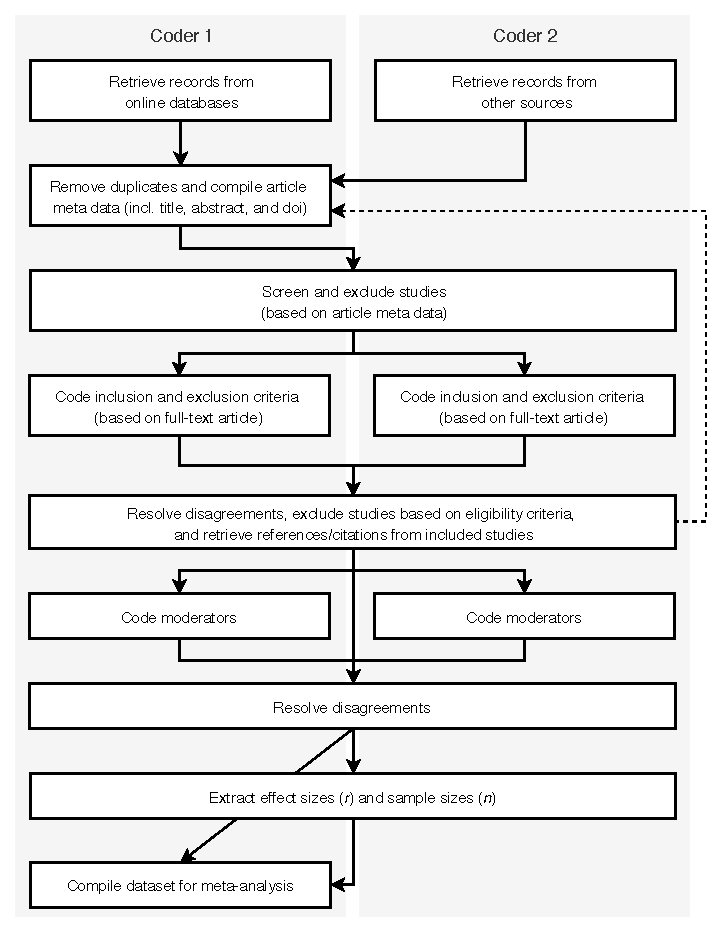
\includegraphics[scale = 1]{coding-diagram}
\caption{Diagram illustrating how two coders search for records, select studies, and collect data for this meta-analysis.}
\label{fig:f1}
\end{figure}

\subsection{Data collection}
\label{sec:data-collection}

We collect the relevant data in two steps. First, we code moderating variables to be used in (exploratory) meta-regression analyses (see Section~\ref{sec:exploratory-analyses}). We decide which moderators to code based on a first review of the included studies. At the very least, we code publication status (\emph{published}, \emph{unpublished}, \emph{unpublished dissertation}), study setting (\emph{ingroup}, \emph{outgroup}, \emph{location}), study design (\emph{cross-sectional}, \emph{longitudinal}, \emph{quasi-experimental}, \emph{experimental}), and study sample (\emph{student}, \emph{community}, \emph{representative}). Two coders each review each of the included full-text manuscripts. We calculate and report inter-rater agreement (Cohen's $\kappa$) for each moderating variable.

% Add additional moderators!

Second, we extract correlation coefficients ($r$) as the relevant measure of effect size, and extract sample sizes ($n$) to calculate standard errors for each sample's correlation coefficients (see Section~\ref{sec:data-synthesis}). Where provided, we copy correlation coefficients from the relevant correlation matrices. Where other effect-size measure are provided, we convert the reported effect sizes to correlation coefficients using common conversion formulas \cite{borenstein_introduction_2009}. Where no effect sizes are provided, we attempt to contact the authors to obtain the relevant correlation matrices or other effect-size measures. If that fails, we impute correlation coefficients from beta coefficients \cite{peterson_beta_2005} if possible.\footnote{$r = \beta + 0.05\lambda$ where $\lambda = 1$ when $\beta \geq 0$ and $\lambda = 0$ when $\beta < 0$ .} If we fail to obtain, calculate, or impute $r$ or $n$ for a sample, we report our failure to do so and exclude the sample from the meta-analysis. At this stage, we also look for samples that might have been reported more than once in the included literature. We consider author names, effect sizes, sample sizes, and other sample characteristics as indicators for duplicate studies. We might contact authors to resolve concerns about the identity of published studies. 

We collect effect sizes for all predictor and outcome variables defined in Section~\ref{sec:eligibility-criteria}, as well as all inter-scale correlations. Where more than one measure is reported, we extract effect sizes for all relevant measures.  In addition, we extract effect sizes for five other measures that might be relevant for exploratory or future analyses: negative contact, ingroup contact, group identification, group-based anger, and outgroup attitudes.

\subsection{Outcome selection}
\label{sec:outcome-selection}

As discussed, we collect data for all relevant predictor and outcome variables defined in Section~\ref{sec:eligibility-criteria}. When a study reports more than one measure of \emph{intergroup contact} (Section~\ref{sec:predictor-variables}), we prioritise the predictor variable in our confirmatory analyses (Section~\ref{sec:confirmatory-analyses}) that measure the most intense or intimate form of contact. We rate contact intensity according to the following ranking: friendship $>$ quality of contact (positive contact) $>$ quantity of contact $>$ opportunity for contact. % that is the focus of the manuscript's primary analysis. If it is unclear what the manuscript's primary analysis is---or if the manuscript's primary analyses considers more than one measure---we combine and average effect sizes across predictor variables. 
If it is unclear which of two predictor variables measures a more intense form of contact, we combine and average effect sizes across these variables. We do not consider negative contact or ingroup contact in our confirmatory analyses. 

When a study reports more than one measure of one or more of the outcome variables defined in Section~\ref{sec:outcome-variables}, we proceed as follows: If a manuscript's primary analysis focuses on one of several \emph{collective action} measure, we prioritise that measure; otherwise, we combine and average effects sizes across outcome variables. If a study reports more than one measure of \emph{policy support}, we combine and average effect sizes for all policies designed to improve the position of the participants' ingroup in society. If a study reports more than one measure of \emph{perceived injustice}, we prioritise the measure closest to perceptions of injustice against the participants' ingroup (rather than against the participants themselves); if it is ambiguous which measure that is, we combine and average effect sizes across outcome variables.

Some study designs result in more than one effect size for the same (combination of) measures. If a \emph{longitudinal} study reports results from more than two waves, we prioritise effect sizes spanning the inter-survey interval closest to one year. If a longitudinal study reports results from more than two waves and spans multiple years, we combine and average effects sizes from each one-year inter-survey interval. In our confirmatory analyses, we focus on the partial correlation between the relevant predictor variable (at time 1) and outcome variable (at time 2) controlling for initial levels of the outcome variable (cross-lagged correlation). If an \emph{experimental} or \emph{quasi-experimental} study reports comparisons between more than two conditions, we prioritise the effect size that compares two conditions that most closely resemble generic contact and no-contact conditions. If it is ambiguous which conditions those are, we combine and average effect sizes comparing experimental conditions to the control condition. We record all decisions about variable selection and data simplification in the published protocol.

\subsection{Data synthesis (meta-analysis)}
\label{sec:data-synthesis}

As discussed, we extract correlation coefficients ($r$) as the relevant measure of effect size. Correlation coefficients, however, are bounded between $-1$ and $1$ and are not suitable for linear regression techniques. Therefore, we convert $r$ to Fisher's $z$, which is unbounded and approximately normally distributed.
\begin{align}
z & = \frac{1}{2} \ln\left(\frac{1 + r}{1 - r}\right) \label{eq:1} \\
\sigma & = \frac{1}{\sqrt{n - 3}} \label{eq:2} \\
r &= \frac{\exp(2z) - 1}{\exp(2z) + 1} = \tanh(z) \label{eq:3}
\end{align}
For each sample, we use equation~\ref{eq:1} to convert $r$ to $z$, and use equation~\ref{eq:2} to calculate the corresponding standard error $\sigma$ from the sample size $n$. We use equation~\ref{eq:3} to convert the effect-size estimates from our meta-analysis back to correlation coefficients.

We estimate Bayesian random-effects meta-analysis models in RStan \cite{rstan_package} using $z$-transformed correlation coefficients as outcome variables:
\begin{align}
z_{ij} &\sim \text{Normal}(\theta_{ij}, \sigma_{ij}) \tag{Likelihood} \\
\theta_{ij} &= 
  \begin{cases} 
    \mu + \textbf{X}\beta_K + \beta_j\tau_J & \text{if } I_j = 1 \\
    \mu + \textbf{X}\beta_K + \beta_j\tau_J + \beta_i\tau_I & \text{if } I_j > 1 
  \end{cases} \tag{Regression}
\end{align}
where $z_{ij}$ is the observed effect size in sample $i$ of study $j$, $\sigma_{ij}$ is the corresponding standard error, and $\theta_{ij}$ is the estimated effect size for sample $i$ of study $j$. We estimate $z_{ij}$ as a function of the estimated mean effect size $\mu$ and, if included, of a matrix $\textbf{X}$ of $K$ observed moderators multiplied by a corresponding vector of $K$ coefficients $\beta_K$. We estimate two varying intercepts, $\beta_i$ and $\beta_j$, with the corresponding standard deviations, $\tau_i$ and $\tau_j$. For studies that contain only one sample ($I_j = 1$), we only estimate $\beta_j$, the study-wise deviation from the mean effect size $\mu$. For studies that contain more than one sample ($I_j > 1$), we also estimate $\beta_i$, the sample-wise deviation from the study-specific effect size. We use the non-centred parameterisation for the varying effects \cite{betancourt_hamilton_2015}. The resulting model is a two-level random-effects meta-analysis. 

Models assigned weakly informative prior distributions \cite{gelman_prior_2017} to all estimated parameters:
\begin{align*} 
\mu &\sim \text{Normal}(0, 0.31605) \\
\beta_i &\sim \text{Normal}(0, 1) \\
\beta_j &\sim \text{Normal}(0, 1) \\
\beta_k &\sim \text{Normal}(0, 1) \\
\tau_I &\sim \text{Half-Cauchy}(0, 0.3) \\
\tau_J &\sim \text{Half-Cauchy}(0, 0.3)
\end{align*}
Figure~\ref{fig:f2} shows the prior distributions for $\mu$, the mean effect size, and $\tau$, the standard deviation of the varying intercepts. The prior distribution for $\mu$ is centred around $0$ and concentrates $50\%$ of the most plausible values between $r = -0.21$ and $r = 0.21$. We focus on $|r| = 0.21$ because it corresponds to the mean effect size observed in both \citeauthor{pettigrew_meta_2006}'s \citeyear{pettigrew_meta_2006} meta-analysis of the contact literature and \citeauthor{richard_meta_2003}'s \citeyear{richard_meta_2003} meta-analysis of effect sizes across a century of social-psychological research. The prior distribution for $\tau$ allocates $30\%$ of plausible values below $\tau = 0.15$. We focus on $\tau = 0.15$ because it corresponds to the standard deviations observed in both \citeauthor{pettigrew_meta_2006}'s \citeyear{pettigrew_meta_2006}\footnote{We estimated $\tau$ in a one-level random-effects meta-analysis using data from \citeA{pettigrew_meta_2006}.} and \citeauthor{richard_meta_2003}'s \citeyear{richard_meta_2003} meta-analyses. We chose this prior distribution following recommendations by \citeA{williams_bayesian_2018}.
 
\begin{figure}
\centering
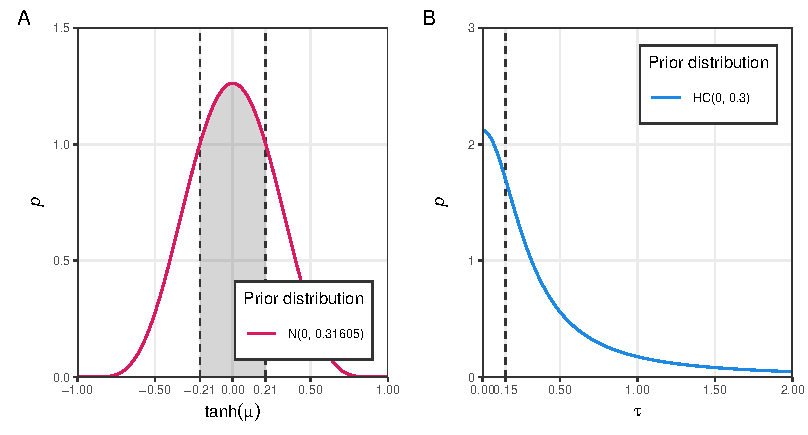
\includegraphics[width = \textwidth]{prior-choice}
\caption{Prior distributions for $\mu$ and $\tau$. (A) Prior distribution for $\mu$ converted from Fisher's $z$ to $r$. The $\text{Normal}(0, 0.31605)$ distribution is centred around $0$ and concentrates $50\%$ of the most plausible values between $r = -0.21$ and $r = 0.21$. (B) Prior distribution for $\tau$. The $\text{Half-Cauchy}(0, 0.3)$ distribution is strictly positive and concentrates $50\%$ of the most plausible values below $\tau = 0.30$.}
\label{fig:f2}
\end{figure}

\subsubsection{Confirmatory analyses}
\label{sec:confirmatory-analyses}

\begin{figure}
\centering
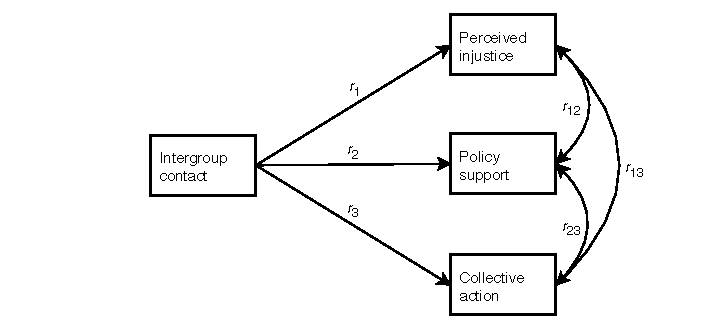
\includegraphics[scale = 1]{path-diagram}
\caption{Path diagram illustrating all correlations that are estimated in our confirmatory analyses.}
\label{fig:f3}
\end{figure}

We conduct confirmatory analyses to answer research questions Q1--Q3 (Section~\ref{sec:objectives}). Specifically, we run six two-level random-effect meta-analysis models (without moderators) to estimate the correlations between intergroup contact and perceived discrimination ($r_1$), policy support ($r_2$), and collective action ($r_3$), as well as the correlations between all three outcome variables ($r_{12}$, $r_{13}$, $r_{23}$), as illustrated in Figure~\ref{fig:f3}. Each model includes only studies/samples that contain the relevant combination of variables. Each model considers predictor and outcome variables as defined in Section~\ref{sec:outcome-selection}.  

\subsubsection{Sensitivity analyses}
\label{sec:sensitivity-analyses}

To assess the robustness of our conclusions, we conduct two kinds of sensitivity analysis. First, we assess to what extent our findings are sensitive to choosing different prior distributions. We repeat the main analyses ($r_{1}$, $r_{2}$, $r_{3}$) with narrower, $\mu \sim \text{Normal}(0, 0.1)$, and wider, $\mu \sim \text{Normal}(0, 1)$, prior distributions. Second, we assess to what extent our findings are sensitive to including or excluding influential studies. We rerun the main analyses $J$ times---leaving out one of $J$ studies each time---and record how much $\mu$, the estimated mean effect size, varies across left-out studies. We calculate the mean absolute error (\textit{MAE}) and compare the study-wise absolute errors ($|\mu_K - \mu_{-k}|$) to identify the most influential studies.
% Third, we assess to what extent our findings are sensitive to studies with large sample sizes. We repeat the main analyses using $\sigma = \frac{1}{\log(n - 3)}$ instead of $\sigma = \frac{1}{\sqrt{n - 3}}$, the correct formula for the standard error. This function decreases much less steeply as $n$ increases, thus reducing the weight of studies with large sample sizes. 
We might report these analyses in an appendix to the published manuscript.

\subsubsection{Exploratory analyses}
\label{sec:exploratory-analyses}

We conduct exploratory analyses to estimate how much the strength of the relevant relationships varies across study designs, study settings, predictor variables, outcome variables, and other (potential) moderating variables. We explore these relationships in a series of two-level random-effect meta-analysis models with moderators. We enter moderating variables with $K$ categories as $K - 1$ mean-centred dummy variables. We run additional meta-analysis models (without moderators) to estimate the partial correlations between the outcome variables and positive/negative contact and ingroup/outgroup contact---if we find enough studies that measure these predictor variables. We consider these analyses exploratory because they are guided by the available data.

\subsection{Meta-biases}
\label{sec:meta-biases}

Publication bias, outcome reporting bias, and (other) questionable research practices in the relevant literature can lead meta-analyses to overestimate effect sizes. Developing methods to detect and correct for such biases is an active area of research, with no available method outperforming all others \cite{carter_correcting_2017}. We assume that the literature underlying our meta-analysis is subject to these meta-biases. We accept that, in lieu of wide-spread adoption of preregistration, detecting and correcting for these biases is difficult or impossible. Nonetheless, we attempt to quantify meta-biases in the relevant literature as follows: First, we test for publication bias by comparing the mean effect sizes of published and unpublished studies. Second, we explore publication bias and other meta biases using statistical methods to detect and correct these biases. We select these methods based on the current state of the literature. We discuss meta-biases as a potential limitation in the published manuscript.

\section{PRISMA-P (2015) checklist}

\figureversion{lining, tabular}
\small
\label{tab:t1}
\begin{tabularx}{\linewidth}{lrX} 
\caption{We explain how this protocol addresses each of the \emph{preferred reporting items for systematic review and meta-analysis protocols} (PRISMA-P; \protect\citeNP{moher_prismap_2015}), and respond to items that we have not yet addressed. \protect\citeA{shamseer_prismap_2015} explain and elaborate all recommended items.} \\
\toprule
Section/Topic~~~~~~~~~~~~~~~~~~~~~ & \# & Response \\ 
\midrule 
\addlinespace 
\endhead
\textit{Administrative information} & & \\ \addlinespace
Title: & & \\
~~~~Identification & 1a & The title identifies the report as the protocol for a meta-analysis.\\
~~~~Update & 1b & This meta-analysis is not an update or extension of any existing systematic review or meta-analysis. \\ \addlinespace
Registration & 2 & This protocol was preregistered with the Open Science Framework on the date stated on the title page. \\ \addlinespace 
Authors: & & \\
~~~~Contact & 3a & To facilitate blind peer review, we do not provide author names or contact information in this preregistered protocol. Below, we refer to the first and second author of the manuscript as A1 and A2.\\
~~~~Contributions & 3b & A1 is the guarantor. A1 and A2 jointly wrote this protocol. A1 contributed the statistical methods to be used in the meta-analysis. A1 and A2 serve, respectively, as Coder~1 and Coder~2 (Figure~\ref{fig:f1}). All authors approved this protocol.
\\ \addlinespace
Amendments & 4 & If we need to amend this protocol, we describe and justify all deviations from this preregistered protocol in the published protocol. \\ \addlinespace
Support: & & \\
~~~~Sources & 5a & No funding has been received for this meta-analysis. We will disclose any future funding received for this meta-analysis. \\
~~~~Sponsor & 5b & N/A \\
~~~~Role of sponsor or funder & 5c & N/A \\ \addlinespace \midrule \addlinespace
\textit{Introduction} & & \\ \addlinespace 
Rationale & 6 & Section~\ref{sec:rationale} summarises the rationale for the meta-analysis. \\ \addlinespace
Objectives & 7 & Section~\ref{sec:objectives} outlines the research questions that the meta-analysis addresses. \\ \addlinespace \midrule \addlinespace
\textit{Methods} & & \\ \addlinespace 
Eligibility criteria & 8 & Section~\ref{sec:eligibility-criteria} spells out all criteria for eligibility for the meta-analysis. \\ \addlinespace 
Information sources & 9 & Section~\ref{sec:information-sources} describes all intended information sources, as well as the planned dates of coverage. \\ \addlinespace 
Search strategy & 10 & Section~\ref{sec:search-strategy} describes our search strategy for four electronic databases, while the planned dates of coverage are described in Section~\ref{sec:information-sources}. \\ \addlinespace
Study records: & & \\
~~~~Data management & 11a & We do not use a dedicated systematic review data management software. We export records from electronic databases as .csv (or similar) files; we import .csv (or similar) files into \emph{R} to compile meta-data and to remove duplicate records \cite{revtools_package}. We use \emph{Qualtrics} and/or \emph{formr} \cite{arslan_formr_2018} surveys to screen and code studies (see Section~\ref{sec:study-selection}). \\
~~~~Selection process & 11b & Section~\ref{sec:study-selection} and Figure~\ref{fig:f1} describe how we select studies for inclusion in the meta-analysis. \\
~~~~Data collection process & 11c & Section~\ref{sec:data-collection} and Figure~\ref{fig:f1} describe how we collect data for each included study/sample. \\ \addlinespace
Data items & 12 & Section~\ref{sec:data-collection} lists all data that is collected; Section~\ref{sec:outcome-selection} explains all pre-planned data simplifications.\\ \addlinespace
Outcomes and prioritization & 13 & Section~\ref{sec:data-collection} describes for which predictor and outcome variables we extract effect sizes; Section~\ref{sec:outcome-selection} explains which predictor and outcome variables are prioritised in our confirmatory analyses.\\ \addlinespace
Risk of bias in individual studies & 14 & We explore study design as a potential source of bias (Section~\ref{sec:exploratory-analyses}). We include all eligible studies in our confirmatory analyses, independent of their risk of bias.\\\addlinespace
Data synthesis & 15a & We will conduct random-effects meta-analyses as described in Section~\ref{sec:data-synthesis}. \\
~~~~ & 15b & Section~\ref{sec:data-synthesis} describes our method for combining data from studies as well as the planned summary methods ($\mu$, $\tau_J$, $\tau_I$). Section~\ref{sec:confirmatory-analyses} proposes confirmatory analyses for answering research questions Q1--Q3.\\
~~~~ & 15c & Sections \ref{sec:sensitivity-analyses} and \ref{sec:exploratory-analyses} propose additional sensitivity and exploratory analyses. \\
~~~~ & 15d & Quantitative synthesis is appropriate for answering research questions Q1--Q3. We will discuss strengths and limitations of the available evidence in a narrative review. \\ \addlinespace
Meta-bias(es) & 16 & Section~\ref{sec:meta-biases} describes our approach to exploring meta-biases in the relevant literature. \\ \addlinespace
Confidence in cumulative evidence & 17 & We do not use a formal approach for assessing the quality of the available evidence, but discuss strengths and limitations of the available evidence in a narrative review.\\
\addlinespace \bottomrule
\end{tabularx}

\bibliographystyle{apacite}
\bibliography{references}

\end{document}